\documentclass[tikz,border=8pt]{standalone}
% Shared look for every TikZ diagram. Load with \input{../../tools/tikz-style.tex}
\usepackage[T1]{fontenc}
\usepackage{lmodern}
\renewcommand{\sfdefault}{lmr}  % diagrams use the same serif as the text
\usetikzlibrary{arrows.meta, positioning, shapes.geometric, calc, fit, backgrounds}
\definecolor{cblue}{HTML}{4C78A8}
\definecolor{corange}{HTML}{F58518}
\definecolor{cgreen}{HTML}{54A24B}
\definecolor{cred}{HTML}{E45756}
\definecolor{cpurple}{HTML}{B279A2}
\definecolor{cgrey}{HTML}{6B6B6B}
\tikzset{
  every picture/.style={font=\sffamily, line width=1.2pt},
  box/.style={draw=#1, fill=#1!12, rounded corners=4pt, align=center, inner sep=7pt, minimum height=1.1cm},
  box/.default=cgrey,
  arrow/.style={-{Stealth[length=3mm]}, draw=cgrey, line width=1.4pt},
  title/.style={font=\sffamily\bfseries\Large},
  note/.style={font=\sffamily\small, text=cgrey, align=center},
}
\AtBeginDocument{\hyphenpenalty=10000 \exhyphenpenalty=10000}

\begin{document}
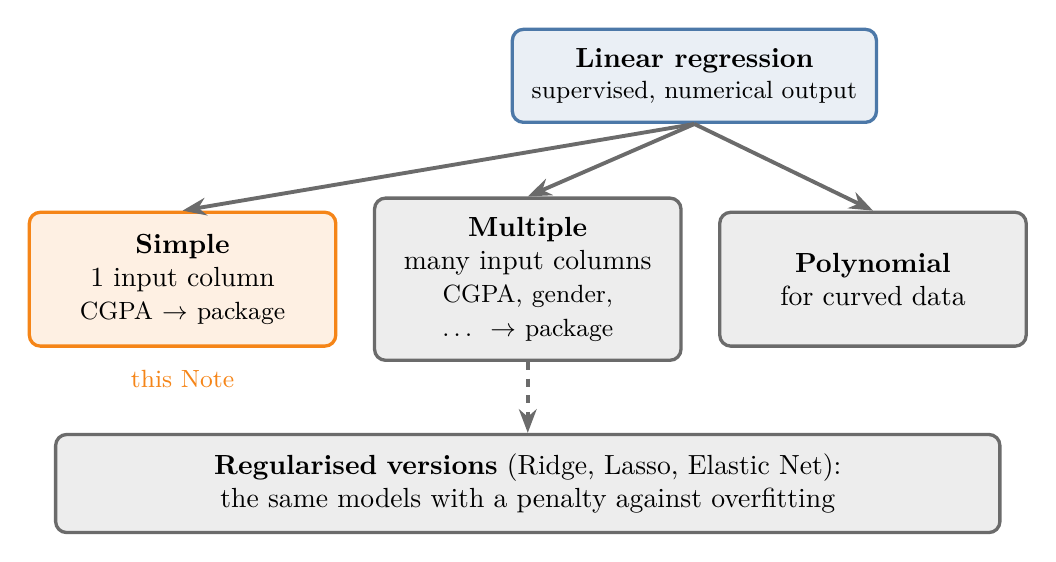
\begin{tikzpicture}[node distance=0.5cm and 0.45cm]
  \node[box=cblue, font=\sffamily\bfseries] (lr) {Linear regression\\[-1pt]\normalfont\small supervised, numerical output};
  \node[box=corange, below left=1.1cm and 2.2cm of lr, text width=3.4cm, minimum height=1.7cm] (s) {\textbf{Simple}\\1 input column\\\small CGPA $\rightarrow$ package};
  \node[box=cgrey, right=of s, text width=3.4cm, minimum height=1.7cm] (m) {\textbf{Multiple}\\many input columns\\\small CGPA, gender, \dots{} $\rightarrow$ package};
  \node[box=cgrey, right=of m, text width=3.4cm, minimum height=1.7cm] (p) {\textbf{Polynomial}\\for curved data};
  \foreach \n in {s,m,p} \draw[arrow] (lr.south) -- (\n.north);
  \node[box=cgrey, below=0.9cm of m, text width=11.5cm] (r) {\textbf{Regularised versions} (Ridge, Lasso, Elastic Net): the same models with a penalty against overfitting};
  \draw[arrow, dashed] (m.south) -- (r.north);
  \node[note, below=0.15cm of s, text=corange] {this Note};
\end{tikzpicture}
\end{document}
